\chapter{Exercise 8}

% ---------------- Exercise 8.1 ----------------
\section{Exercise 8.1}
\subsection{Problem}
Given the translation scheme for the EQN language (see pp.\,40 in this lecture), calculate the height and depth of the input:
\[
\texttt{text sub text sub text}.
\]
Suppose that for each \texttt{text},
\begin{itemize}
    \item $\mathrm{getHeight}(ps, \texttt{text.lexval}) = 8 \times ps$,
    \item $\mathrm{getDepth}(ps, \texttt{text.lexval}) = 0$.
\end{itemize}

\begin{figure}
\centering
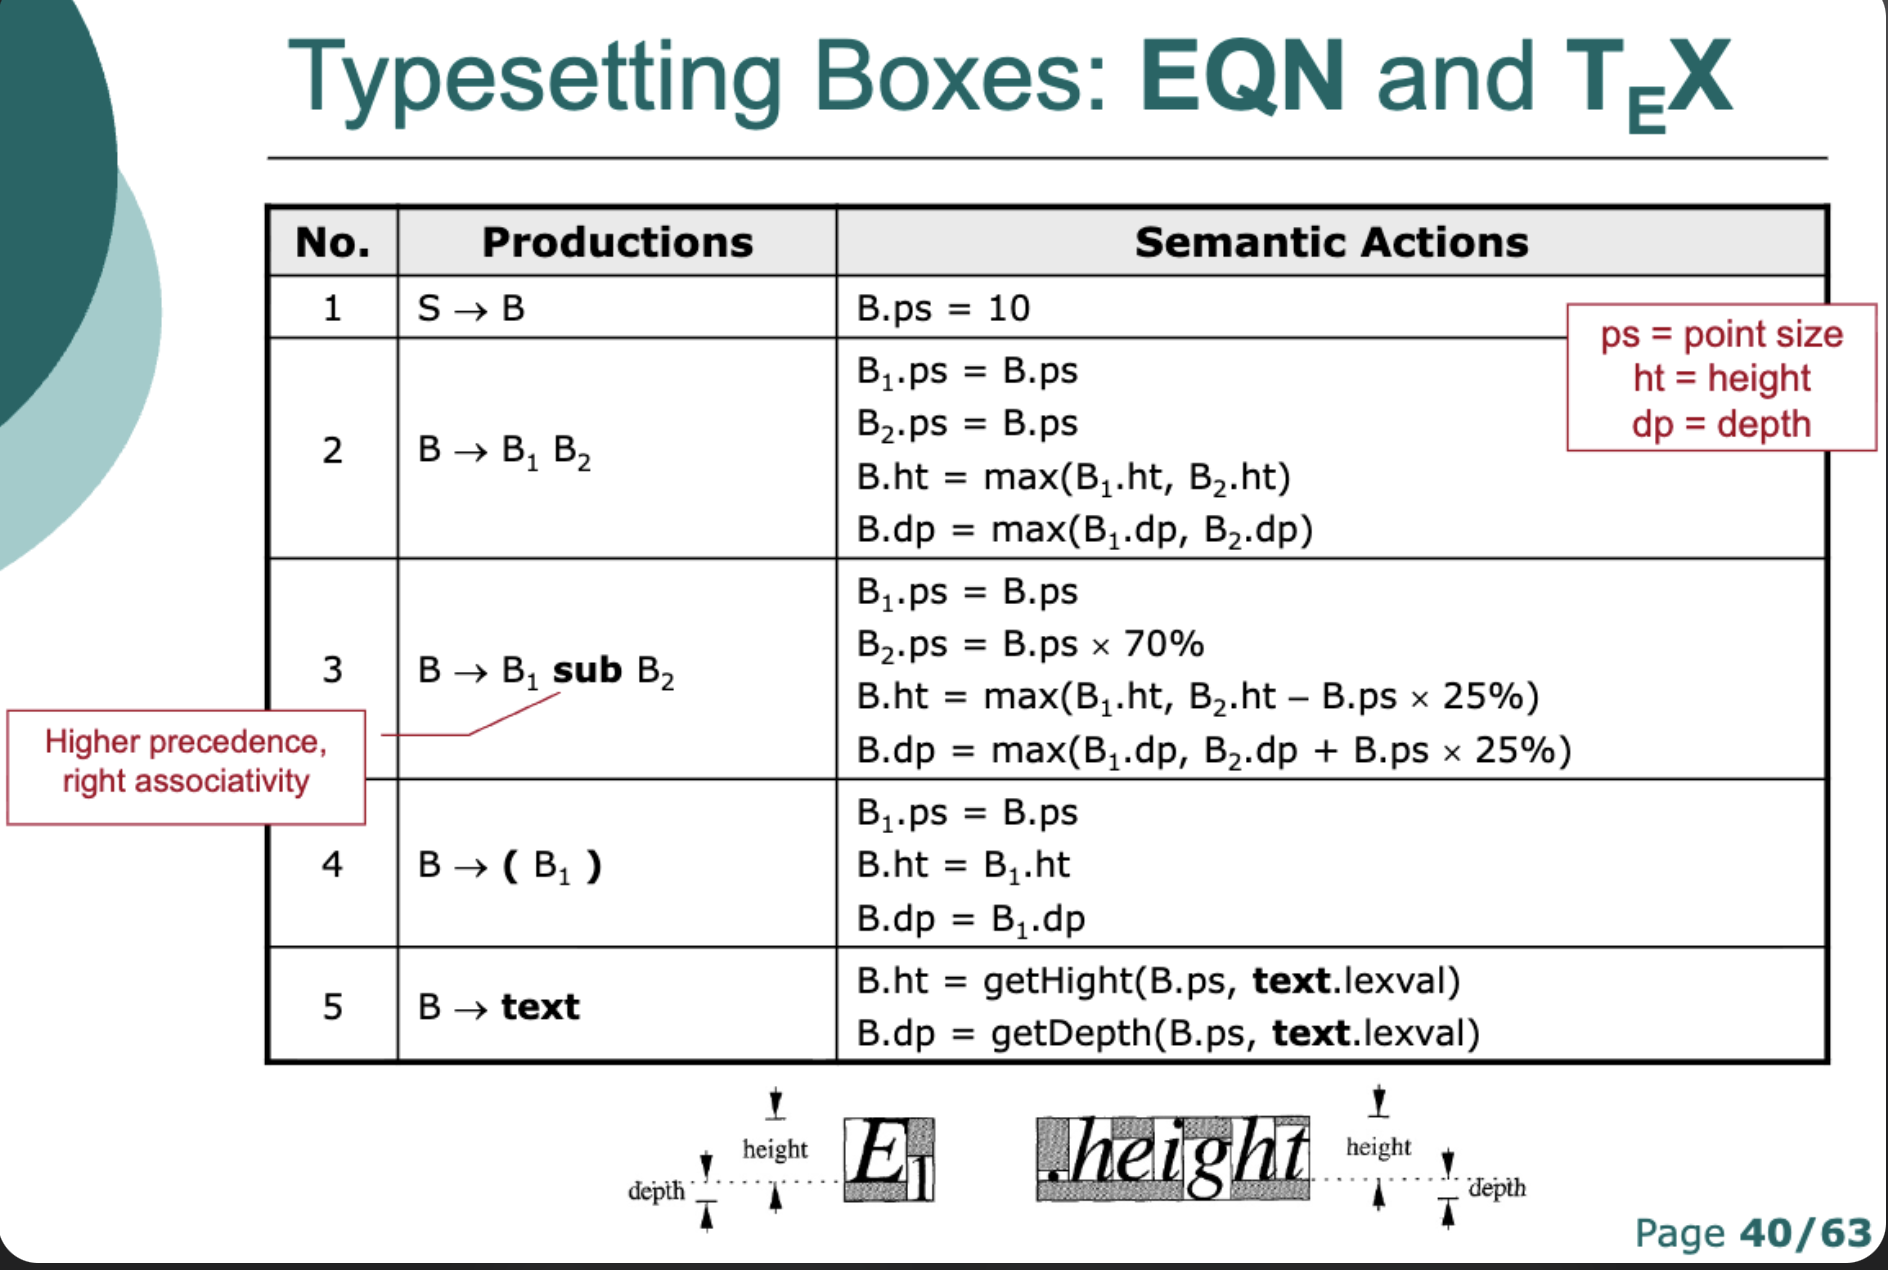
\includegraphics[width=0.7\textwidth]{image/rule.png}
\end{figure}


\newpage
\subsection{Solution}

% TODO
We compute attributes bottom-up using the semantic rules on Page 40/63.

The input \texttt{text sub text sub text} is parsed as right-associative:
\[
\texttt{text sub (text sub text)}
\]
Corresponding parse tree (nonterminals labeled as in the grammar):
\begin{center}
\begin{tikzpicture}[level distance=20mm,
  level 1/.style={sibling distance=60mm},
  level 2/.style={sibling distance=30mm},
  level 3/.style={sibling distance=20mm},
  every node/.style={font=\footnotesize}]
  \node {S}
    child {node {B}
      child {node {B$_1$}
        child {node {text}}
      }
      child {node {sub}}
      child {node {B$_2$}
        child {node {B$_3$}
          child {node {text}}
        }
        child {node {sub}}
        child {node {B$_4$}
          child {node {text}}
        }
      }
    };
\end{tikzpicture}
\end{center}

Now apply semantic actions:

\begin{enumerate}
    \item Rule 1: $S \to B$ gives $B.\mathit{ps} = 10$.

    \item Rule 3 ($B \to B_1\ \texttt{sub}\ B_2$):
    \begin{itemize}
        \item $B_1.\mathit{ps} = B.\mathit{ps} = 10$,
        \item $B_2.\mathit{ps} = B.\mathit{ps} \times 70\% = 10 \times 0.7 = 7$.
    \end{itemize}

    \item Rule 5 ($B_1 \to \texttt{text}$):
    \begin{itemize}
        \item $B_1.\mathit{ht} = 8 \times B_1.\mathit{ps} = 8 \times 10 = 80$,
        \item $B_1.\mathit{dp} = 0$.
    \end{itemize}

    \item Rule 3 applied to $B_2 \to B_3\ \texttt{sub}\ B_4$:
    \begin{itemize}
        \item $B_3.\mathit{ps} = B_2.\mathit{ps} = 7$,
        \item $B_4.\mathit{ps} = B_2.\mathit{ps} \times 70\% = 7 \times 0.7 = 4.9$.
    \end{itemize}

    \item Rule 5 for leaves:
    \begin{itemize}
        \item $B_3.\mathit{ht} = 8 \times 7 = 56$, \quad $B_3.\mathit{dp} = 0$,
        \item $B_4.\mathit{ht} = 8 \times 4.9 = 39.2$, \quad $B_4.\mathit{dp} = 0$.
    \end{itemize}

    \item Rule 3 for $B_2$ (synthesized attributes):
    \begin{align*}
        B_2.\mathit{ht} &= \max\bigl(B_3.\mathit{ht},\; B_4.\mathit{ht} - B_2.\mathit{ps} \times 25\%\bigr) \\
                        &= \max\bigl(56,\; 39.2 - 7 \times 0.25\bigr) = \max(56,\; 39.2 - 1.75) = \max(56,\; 37.45) = 56, \\
        B_2.\mathit{dp} &= \max\bigl(B_3.\mathit{dp},\; B_4.\mathit{dp} + B_2.\mathit{ps} \times 25\%\bigr) \\
                        &= \max\bigl(0,\; 0 + 1.75\bigr) = 1.75.
    \end{align*}

    \item Finally, Rule 3 for the top-level $B$:
    \begin{align*}
        B.\mathit{ht} &= \max\bigl(B_1.\mathit{ht},\; B_2.\mathit{ht} - B.\mathit{ps} \times 25\%\bigr) \\
                      &= \max\bigl(80,\; 56 - 10 \times 0.25\bigr) = \max(80,\; 53.5) = \boxed{80}, \\
        B.\mathit{dp} &= \max\bigl(B_1.\mathit{dp},\; B_2.\mathit{dp} + B.\mathit{ps} \times 25\%\bigr) \\
                      &= \max\bigl(0,\; 1.75 + 10 \times 0.25\bigr) = \max(0,\; 4.25) = \boxed{4.25}.
    \end{align*}
\end{enumerate}

Thus, the height of the expression is $80$ and the depth is $4.25$.